\documentclass[10pt,twoside,a4paper]{article}

% Configure these parameters.
% Name and email
\newcommand{\studentname}{Joe Yan}
\newcommand{\studentemail}{zy275@cam.ac.uk}

% Date work done
\newcommand{\svworkdate}{2017-1-22}

% Details of supervision
\newcommand{\svcourse}{CST Part IA: Algorithm}
\newcommand{\svnumber}{1}
\newcommand{\svdate}{2016-2-3}
\newcommand{\svtime}{1500}
\newcommand{\svvenue}{Churchill 1C}
\newcommand{\svrname}{Dr John Fawcett}
\newcommand{\svrinit}{JKF}
% End configuration

\usepackage{a4}             % Adjust margins for A4 media
\usepackage{pgfplots}
\usepackage{fancyhdr}
\renewcommand{\headrulewidth}{0.4pt}
\renewcommand{\footrulewidth}{0.4pt}
\fancyheadoffset[LO,LE,RO,RE]{0pt}
\fancyfootoffset[LO,LE,RO,RE]{0pt}
\pagestyle{fancy}
\fancyhead{}
\fancyhead[LO,RE]{{\bfseries \studentname}\\\studentemail}
\fancyhead[RO,LE]{{\bfseries \svcourse, SV~\svnumber}\\\svdate\ \svtime, \svvenue}
\fancyfoot{}
\fancyfoot[LO,RE]{For: \svrname}
\fancyfoot[RO,LE]{\thepage\ / \pageref{LastPage}}
\fancyfoot[C]{\today}

\usepackage{lastpage}       % "n of m" page numbering
\usepackage{lscape}         % Makes landscape easier
%\usepackage{portland}      % Switch between portrait and landscape
\usepackage{graphics}       % Graphics commands
\usepackage{wrapfig}        % Wrapping text around figures
\usepackage{epsfig}         % Embed encapsulated postscript
\usepackage{rotating}       % Extra graphics rotation
%\usepackage{tables}        % Tabular environments
\usepackage{longtable}      % Page breaks within tables
\usepackage{supertabular}   % Page breaks within tables
\usepackage{multicol}       % Allows table cells to span cols
\usepackage{multirow}       % Allows table cells to span rows
\usepackage{texnames}       % Macros for common tex names
%\usepackage{trees}         % Tree-like layout
\usepackage{hhline}         % Horizontal lines in tables
\usepackage{siunitx}        % Correct spacing of units

\usepackage{listings}       % Source code listings
\usepackage{array}          % Array environment
\usepackage{hyperref}       % URL formatting
\usepackage{amsmath}        % American Mathematical Society
\usepackage{amssymb}        % Maths symbols
\usepackage{amsthm}         % Theorems
%\usepackage{mathpartir}    % Proofs and inference rules
\usepackage{verbatim}       % Verbatim blocks
\usepackage{ifthen}         % Conditional processing in tex
\usepackage{xcolor}         % X11 colour names

% control width and vertically align text in table cells
\newcolumntype{L}[1]{>{\raggedright\let\newline\\\arraybackslash\hspace{0pt}}m{#1}}
\newcolumntype{C}[1]{>{\centering\let\newline\\\arraybackslash\hspace{0pt}}m{#1}}
\newcolumntype{R}[1]{>{\raggedleft\let\newline\\\arraybackslash\hspace{0pt}}m{#1}}

% make hyperref links not-ugly
\hypersetup{
    colorlinks=false,
    pdfborder={0 0 0},
}

\renewcommand{\oddsidemargin}{-20pt}
\renewcommand{\evensidemargin}{-20pt}
\renewcommand{\topmargin}{-30pt}
\renewcommand{\textwidth}{410pt}
\renewcommand{\marginparwidth}{100pt}

\setlength{\parindent}{0em}
\addtolength{\parskip}{1ex}

\usepackage[draft]{changes}
\setauthormarkup[left]{\textbf{[#1]}~}
\definechangesauthor[\svrname]{\svrinit}{orange}
\newcommand{\jkfadd}[1]{\added[\svrinit]{#1}}
\newcommand{\jkfdel}[1]{\deleted[\svrinit]{#1}}
\newcommand{\jkfrep}[2]{\replaced[\svrinit]{#1}{#2}}
\newcommand{\jkfmar}[1]{\marginpar{\jkfadd{#1}}}

\begin{document}

\author{\studentname}
\title{\svcourse, SV~\svnumber}
\date{\svworkdate}

\textbf{\svcourse, SV~\svnumber}\\
\textbf{\studentname}\\
\textbf{\svworkdate}\\

\section{2009P1Q6}
\begin{itemize}
\item[(a)]
The value at position k is smaller or equal to values at position 2k+1 and 2k+2.\\
The tree must be a almost full binary tree. It must have maximum number of nodes and its last level must either be full or have empty spaces only at its right end.\\
\begin{lstlisting}
         0
    1         2
 3    4    5    6
7 8  9 10 ....
\end{lstlisting}
\item[(b)]
It is a ascending sorted array so it is a full binary tree. (there are no holes in the array)\\
$$\forall \ ascending\  Array[]\ a<b\ in\ index\ range. Array[a]\leq Array[b]$$
$$\forall k\in \mathbb{N}_0.k<2k+1<2k+2$$
So we can say $\forall k\in \mathbb{N}_0, \ ascending\  Array[]\ a<b\ in\ index\ range. Array[k]\leq Array[2k+1]\leq Array[2k+2]$\\
Such arrays satisfy both property of min-heap so it is a min-heap.
\item[(c)]
Without lost of generality: AIERPMSNL - 132875964\\
The 8 at position 3 is larger than 4 at position $8=2\cdot 3 +2$. So it is not a min-heap.\\
Here we heapify with root from position 3 to position 0.\\
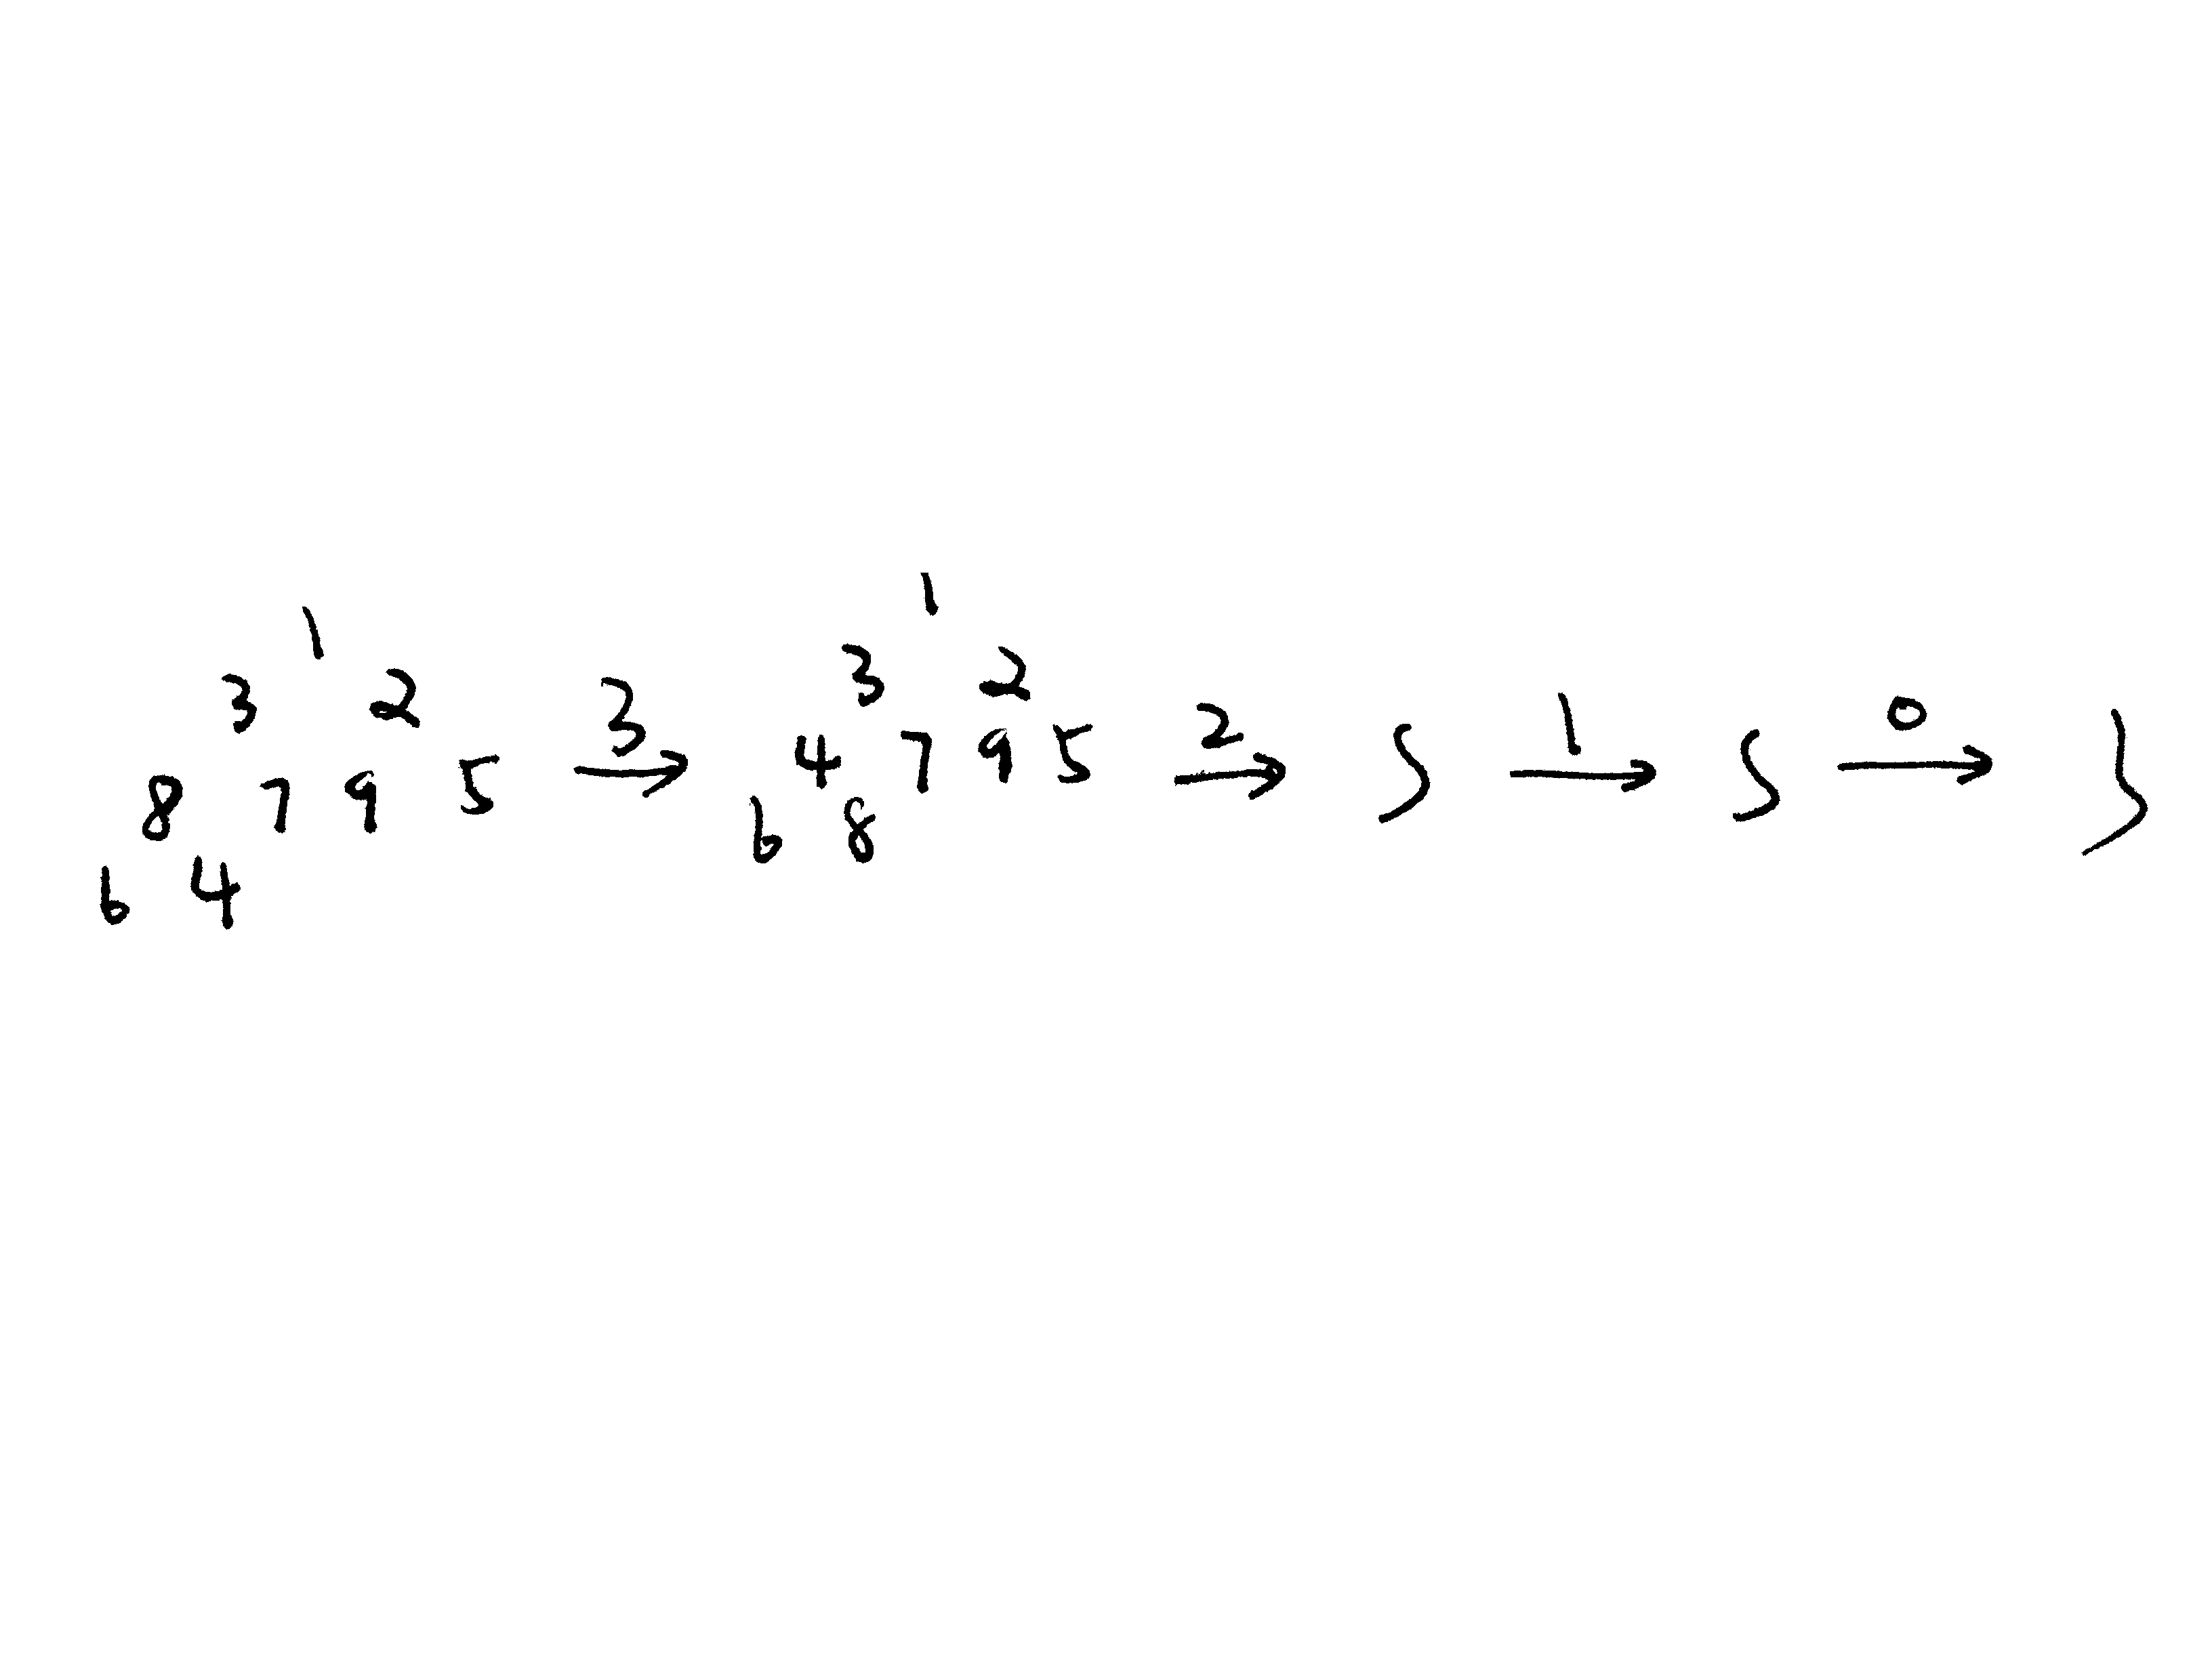
\includegraphics[scale=0.1]{SV2a.png}
Heapify with root at 3 change the 8 at position 3 with its smallest child 4 at position 8.\\
Heapify with root at (2,1,0) do nothing to the data because it is already a min-heap.
\item[(d)]

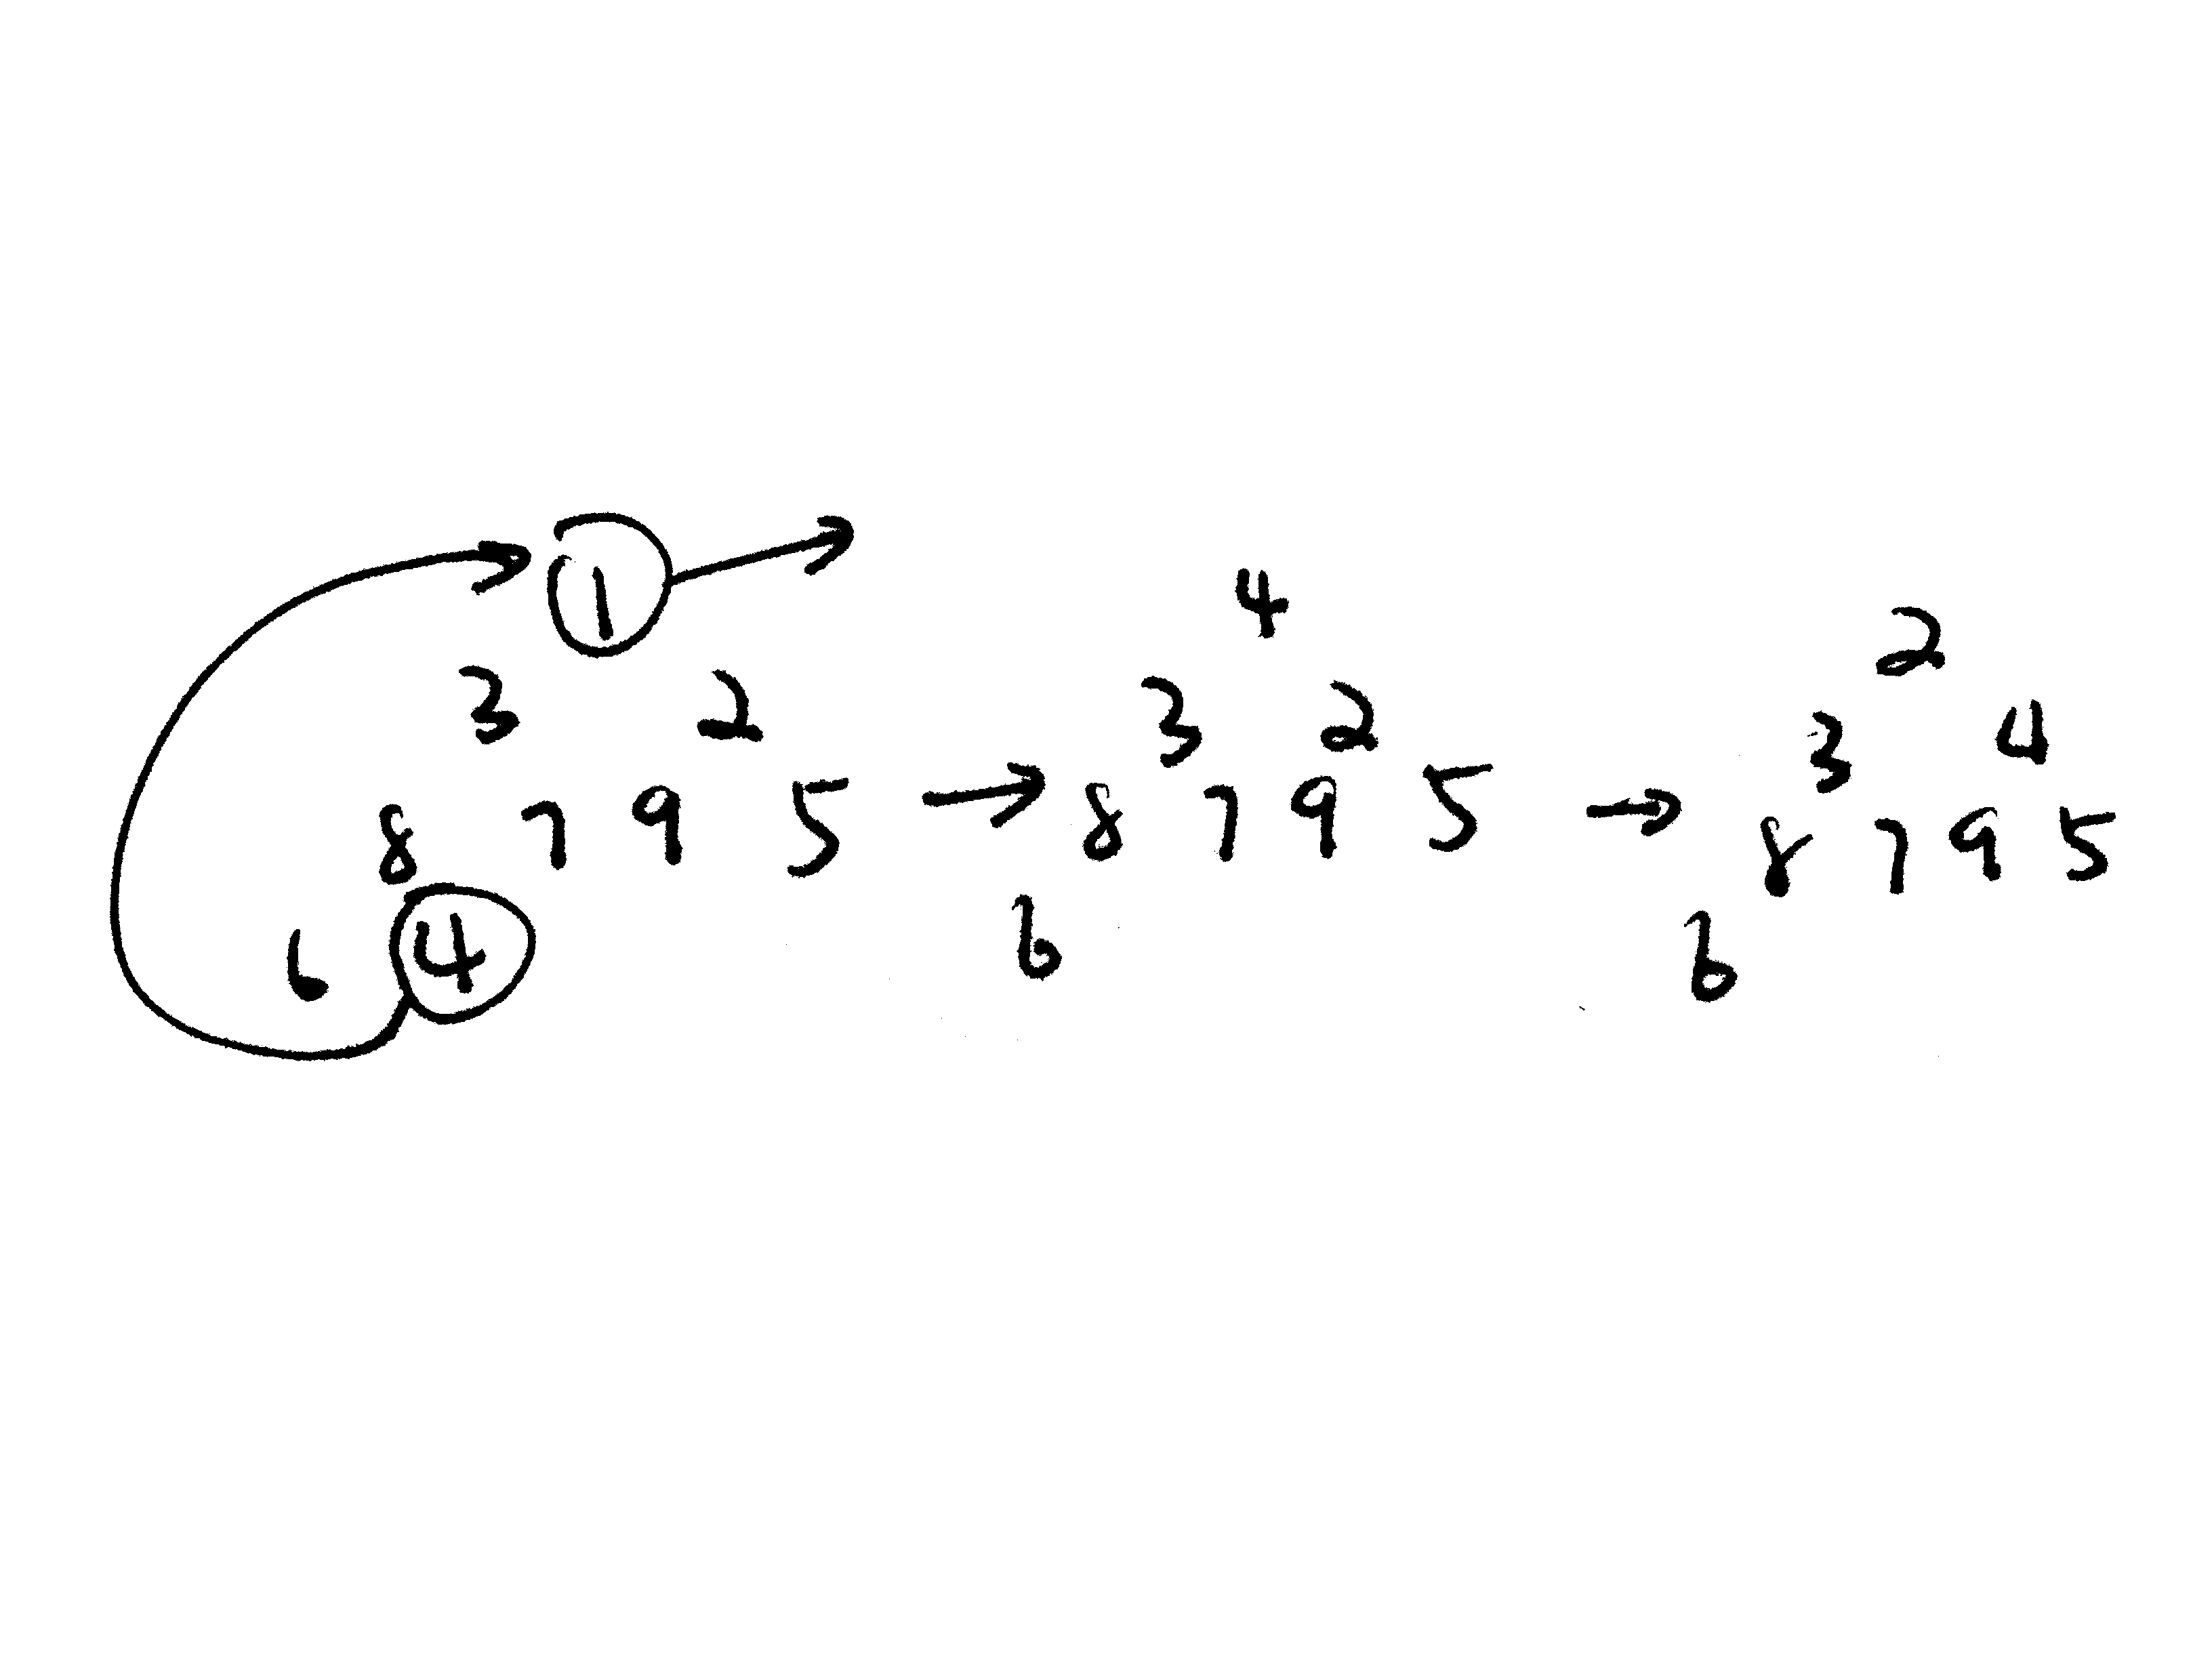
\includegraphics[scale=0.1]{SV2b.png} 
After remove the smallest element 1, move 4 which was at the end of the heap to the top.\\
Heapify with root at 0 will rearrange the heap and make it a min-heap again.
\item[(e)]
$$O(n\log n)$$
Let the time cost to be f(n) for heapify() with a length n heap.
$$f(n)=f(n/2)+k$$
$$f(n)=k\log n$$
In heapsort, the first step is to make a max-heap by call heapify from position n/2 floor to 0.\\
Let the time cost to be A(n) for this stage.\\
$$A(n)=\Sigma_{i=n/2}^{n}f(i)=\Sigma_{i=n/2}^{n}k\cdot \log i =O(n\log n)$$
The second step is keep swapping the largest element in the heap  with the last element in the heap. Now the size of heap reduce by one and call heapify() to maintain the property of heap. Repeating doing so, the array will finally end up with ascending order again.\\
Let the time cost to be B(n) for this stage.\\
$$B(n)=B(n-1)+f(n-1)=\Sigma_{i=0}^{n-1}f(i)=\Sigma_{i=0}^{n-1}O(\log i)=O(n\log n)$$
Overall the time complexity will be $A(n)+B(n)$ which is $O(n\log n)$
\item[(f)]
$$O(n\log n)$$
This time the input array is already a max-heap so the time complexity for making a max-heap will be neglectable compare with later maintaining the max-heap while swapping the max element with the last element of the heap. B(n) dominants the time complexity which is $O(n/log n)$
\end{itemize}
\section{2010P10Q10}
\begin{itemize}
\item[(a)]
\begin{lstlisting}
partition(arr[],beg,end){
left=beg
right=end-1
p=arr[end]
while(left != right){
	if(left <= p) ++left
	else swqp(arr[],left,right)
		   --right
}
if(left <= p) swqp(arr[],left+1,end)
	else swqp(arr[],left,end)
return left
}
ith(arr[],beg,end,i){ //i means index i
p=partition(arr[],beg,end)
if(p=i) return p
else if(p<i) ith(arr[],p+1,end)
       else ith(arr[],beg,p-1)
}
\end{lstlisting}
Let the time cost to be f(n) for finding ith element in an unordered array with size n.
$$f(n)=f(m)+kn \  (m\in [1,n])$$
$$f(n)=O(n)$$
We can also sort the array and pick the ith element directly by index. However this is less efficient ($O(n\log n)$) than the method above.\\
\item[(b)]
\begin{itemize}

\item
We are finding k smallest elements in a very large array with size n. The best way is to maintain a small array with size k at the begin of the input array (for in place). While go through the whole array check whether the element is smaller than the largest element in the small array. If it is smaller than swap them, otherwise leave them. Finally return arr[0,k-1] which are required elements.The worst time complexity should be $O(kn)$ on average it will be $O(n\log k)$ (using binary insertion), if k is small compare to n, it is definitely better than $O(n\log n)$.\\
\item
We can also use almost exactly the same method as (a) to find the k smallest elements under the assumption of all elements are distinct.\\
Notice for each pivot we called with partition(), the algorithm divides the array to regions separated by picked pivot and the value of elements between two pivot  should always be between them if there are no equal tests can return true.\\
As we find ith element, instead of return ith element, we return arr[0:p-1] in the ith. As we argued, all elements in arr[0,p-1] are smaller than arr[p] which is the ith smallest element in the array. So we find the k smallest elements in the input array with average time complexity $O(n)$. However, the worse-case time complexity is $O(n\log n)$ which is worse than the first idea.\\
\item
As the question said we can call ith() for k times but its unnecessary as argued before, k times more time cost.
\item
We can also sort the array first with time complexity $O(n\log n)$.
\end{itemize}
\item[(c)]
Use the idea of divide and conquer, the algorithm compares the position 1 and 2, 3 and 4... and take the smaller elements to form a new array and repeat the process again. Finally we will end up with a singleton which is the smallest element we want.\\
Let f(n) be the time of comparison needed for an array with size n.
$$f(n)=
\begin{cases}
f(n/2)+n/2,2 | n\\
f((n+1)/2)+(n-1)/2,2\not| n
\end{cases}$$
To calculate this recursion notice under both cases ($i<k,n_i<n_k$):
$$f(1)=0$$
$$f(n_0)=f(n_1)+(n_0-n_1)$$
From the equation above we have:
$$f(n_0)=f(n_1)+(n_0-n_1)=f(n_2)+(n_1-n_2)+(n_0-n_1)=...=f(1)+n-1=n-1$$
The number of comparisons under worst-case (actually for all case) will be the same for the first method in (b) but the method in  (c) is not searching in place so actually a worse idea.
\item[(d)]
Consider this as a tournament as how we found the smallest element in (c). The second smallest element can only be in the set of element that is beaten by the smallest element assuming no duplication. So in the worst-case, the cardinality of such set is precisely $\lceil\log_2n\rceil$. To find the smallest element in this set takes $\lceil\log_2n\rceil -1$ comparison as argued in (c).\\
Overall, it takes $n+\lceil\log_2n\rceil -2$ comparison in the worst case.
\end{itemize}
\end{document}

